%\documentclass[11pt]{book}
\documentclass[graybox]{svmult}

\usepackage[british]{babel}
%\usepackage[garamond]{mathdesign}

%\usepackage{authblk}

\usepackage{mathptmx}       % selects Times Roman as basic font
\usepackage{helvet}         % selects Helvetica as sans-serif font
\usepackage{courier}        % selects Courier as typewriter font
%\usepackage{type1cm}        % activate if the above 3 fonts are
                             % not available on your system

\usepackage{makeidx}         % allows index generation
\usepackage{graphicx}        % standard LaTeX graphics tool
                             % when including figure files
\usepackage{multicol}        % used for the two-column index
\usepackage[bottom]{footmisc}% places footnotes at page bottom


\usepackage{hyperref,url}

\usepackage{mathptmx}
\usepackage{amsmath}
\usepackage{courier}
\usepackage{amssymb}
\usepackage{mathtools}

\let\proof\relax\let\endproof\relax

\usepackage{amsthm}

\usepackage{enumerate}
\usepackage{enumitem,multicol}
\usepackage{tikz}
\usepackage{nicefrac}
\usepackage{bm}
\usepackage{algorithm}
\usepackage{algorithmicx}
\usepackage{algpseudocode}

\usepackage{graphicx}
\usepackage{caption}

%\usepackage{eufrak}

%\usepackage{hyperref}
%\usepackage{pdfsync}
%\usepackage{authblk}

\DeclareMathAlphabet\mathbfcal{OMS}{cmsy}{b}{n}

%\theoremstyle{definition}
%\newtheorem{exmp}{Example}%[section]
 
%\renewcommand{\ttdefault}{cmtt}
%\newtheorem{theorem}{Theorem}
%\newtheorem{proposition}[theorem]{Proposition}
%\newtheorem{corollary}[theorem]{Corollary}
%\newtheorem{lemma}[theorem]{Lemma}
%\newtheorem{definition}{Definition}

%\newtheorem{remark}{Remark}
%\newtheorem*{remark*}{Remark}

%\newtheorem{claim}{Claim}[theorem]
%\newtheorem*{claim*}{Claim}


\algrenewcommand\algorithmicrequire{\textbf{Input:}}
\algrenewcommand\algorithmicensure{\textbf{Output:}}

% - macros

\newcommand{\nats}{\mathbb{N}}
\newcommand{\natswith}{\nats_{0}}
\newcommand{\reals}{\mathbb{R}}

\newcommand{\realspos}{\reals_{>0}}
\newcommand{\realsnonneg}{\reals_{\geq 0}}

\newcommand{\states}{\mathcal{X}}
\newcommand{\observs}{\mathcal{Y}}

\newcommand{\paths}{\Omega}
%\newcommand{\path}{\omega}

\newcommand{\power}{\mathcal{P}(\paths)}
\newcommand{\nonemptypower}{\power_{\emptyset}}
\newcommand{\events}{\mathcal{E}}
%\newcommand{\nonemptyevents}{\events^{\emptyset}}
\newcommand{\filter}[1][t]{\mathcal{F}_{#1}}
\newcommand{\eventst}[1][t]{\events_{#1}}

\newcommand{\processes}{\mathbb{P}}
\newcommand{\mprocesses}{\processes^{\mathrm{M}}}

\newcommand{\hmprocesses}{\processes^{\mathrm{HM}}}

\newcommand{\wprocesses}{\processes^{\mathrm{W}}}
\newcommand{\wmprocesses}{\processes^{\mathrm{WM}}}

\newcommand{\whmprocesses}{\processes^{\mathrm{WHM}}}

\newcommand{\lexp}{\underline{\mathbb{E}}_{\rateset,\mathcal{M}}}
\newcommand{\uexp}{\overline{\mathbb{E}}_{\rateset,\mathcal{M}}}

\newcommand{\lt}{\underline{T}}
\newcommand{\lbound}{L}

\newcommand{\gambles}{\mathcal{L}}
\newcommand{\gamblesX}{\gambles(\states)} 

\newcommand{\ind}[1]{\mathbb{I}_{#1}}

\newcommand{\rateset}{\mathcal{Q}}
\newcommand{\lrate}{\underline{Q}}

\newcommand{\asa}{\Leftrightarrow}
\newcommand{\then}{\Rightarrow}

\newcommand{\norm}[1]{\left\lVert #1 \right\rVert}
\newcommand{\abs}[1]{\left\vert #1 \right\vert}

\newcommand{\coloneqq}{:\!=}

\newcommand{\opinset}{\,\,\widetilde{\in}\,\,}

\newcommand{\argmin}{\arg\min}

\newcommand{\exampleend}{\hfill$\Diamond$}

\newcommand{\ictmc}{{ICTMC}}

\newcommand{\prev}{\bbbe}

\newcommand{\timedim}{\mathbb{T}}

\def\presuper#1#2%
  {\mathop{}%
   \mathopen{\vphantom{#2}}^{#1}%
   \kern-\scriptspace%
   #2}

\makeatletter
\newcommand{\customlabel}[2]{%
   \protected@write \@auxout {}{\string \newlabel {#1}{{#2}{\thepage}{#2}{#1}{}} }%
   \hypertarget{#1}{\emph{#2}\!}
}
\makeatother


\usepackage{color,soul,booktabs}
\setulcolor{blue}
\newcommand{\BibTeX}{\textsc{B\kern-0.1emi\kern-0.017emb}\kern-0.15em\TeX}

\makeindex

\begin{document}

% Running title and authors 
%\ShortHeadings{Efficient Computation of Updated Lower Expectations for ICTHMC's}{Krak et al.} 

\title{Imprecise Markov Chains}
% Use \titlerunning{Short Title} for an abbreviated version of
% your contribution title if the original one is too long
\author{Thomas Krak}
% Use \authorrunning{Short Title} for an abbreviated version of
% your contribution title if the original one is too long
\institute{Thomas Krak \at IDLab, Ghent University, \email{thomas.krak@ugent.be}
}
%
% Use the package "url.sty" to avoid
% problems with special characters
% used in your e-mail or web address
%
\maketitle

\abstract{This is a placeholder abstract.
}

%\chapter{Imprecise Markov Chains}

\section{Introduction}

In many areas of science and engineering, we are interested in modelling uncertainty about (the behaviour of) dynamical systems, that is, systems whose state changes as time elapses.

{\bf TODO: some examples relevant to UTOPIAE. Trajectory tracking, reliability/failure analysis etc. Some other examples with broader scope.}

Our uncertainty about the behaviour of such a system can be due to various reasons. For example, there may be an intrinsically stochastic component to the system under study. Regardless of the interpretation that we want to assign to this kind of uncertainty, systems of this kind are modelled using \emph{stochastic processes}. {\bf TODO: bit more explanation and intuition.}

On the other hand, we might also be uncertain about whether our model is correct. For instance, we might not know exactly the numerical values that the parameters of our model should take. Similarly, we might be aware that our modelling assumptions lead to simplifications that are not necessarily warranted, which introduces uncertainty about the accuracy or applicability of any assessments made on the basis of these models. It is therefore of interest to robustify our models also against these kinds of ``meta'', or ``higher-order'', uncertainties.

In this chapter, we consider stochastic processes for which this higher-order uncertainty is modelled using the theory of Imprecise Probabilities (IP). For an extended introduction to IP, we refer the reader back to Chapter {\bf REF}. We here constrain ourselves to briefly recall that such Imprecise Probabilistic models can be interpreted as representing a \emph{set} of traditional probabilistic models. So, in our current setting, we will be considering \emph{sets} of stochastic processes. From an inference point of view, the aim is then to compute inferences which are robust with respect to variations within such a set. We recall from Chapter {\bf REF} that these robust inferences are captured in general by the \emph{lower} and \emph{upper} expectations with respect to the elements of the set that we are considering.

Our aim with the present chapter is to provide an extensive but intuitive overview of the theory of Imprecise Stochastic Processes, and of Imprecise Markov Chains in particular. To this end, we will intentionally focus on different representations of these processes. We will show how each of these different ways of looking at these models provides its own way of deriving useful properties and highlights different intuitive ways of reasoning about them. Important results and properties are stated, but we have made an effort to keep the discussion intuitive. We try to prevent technicalities and do not provide extended proofs; instead, we provide pointers to the literature that the interested reader might pursue herself.

{\bf TODO: The remainder of this chapter is structured as follows...}

\section{(Precise) Stochastic Processes}

%\emph{In this section: Some notation and formalisation. Different representations; probability measures (intuitively, not going to do the full measure theoretic treatment), event trees, graphical models (again: short, not the full general theory). Various independence concepts, and Markov chains as a special case. Computations using law of iterated expectation. Focus largely on discrete-time, with some first concepts about continuous-time. A brief discussion about limit behaviour.}

We will start the exposition around stochastic processes in a relatively general and abstract sense, but will quickly make things more specific. Throughout the remainder of this chapter, we will consider some fixed abstract \emph{state-space} $\states$. A \emph{state} is an element $x\in\states$ and represents uniquely the relevant information about the underlying system that we are interested in modelling. So as not to complicate matters, we will assume throughout that $\states$ is finite, so that we can identify it without loss of generality as the set $\states=\{1,\ldots,k\}\subset\nats$. Note that here and in what follows, we denote with $\nats$ the natural numbers, and will write $\natswith\coloneqq\nats\cup\{0\}$ when we include zero. Furthermore, the real numbers are written $\reals$, the non-negative reals are $\realsnonneg$, and the positive reals are $\realspos$.

Because we are interested in modelling a system whose state $x\in\states$ changes over time, we next identify some \emph{time-dimension} $\timedim$. A crucial choice to be made later on is whether we are considering processes in discrete-time, in which case we identify $\timedim=\natswith$, or processes in continuous-time, in which case $\timedim=\realsnonneg$. For now we simply keep the discussion general without making this identification.

With the state-space and time-dimension in place, it now makes sense to talk about the \emph{realisation} of some (yet to be identified) stochastic process. Such a realisation is also called a \emph{sample path}, and it is a function $\omega:\timedim\to\states$. So, this $\omega$ describes for each point in time $t\in\timedim$ the state $\omega(t)\in\states$ that the system was in at that time. We collect in the set $\Omega$ all these sample paths. For technical reasons, it is sometimes required to restrict attention to paths that satisfy sufficient smoothness conditions; for instance, when $\timedim=\realsnonneg$ it is common practice to let $\Omega$ only contain c\`adl\`ag functions, that is, paths $\omega(t)$ that are right-continuous and whose left-sided limits exists everywhere.

This set $\Omega$ thus contains all possible ways in which the system might behave over time; it can therefore be considered an \emph{outcome space} of a stochastic model. Formally, we will consider some abstract underlying probability space $(\Omega,\mathcal{F},P)$, where $\mathcal{F}$ is some appropriate $\sigma$-algebra on $\Omega$ and where $P$ is a probability measure on $(\Omega,\mathcal{F})$. Given this probability space, we can finally formalise the notion of a \emph{stochastic process} as a collection $\{X_t\}_{t\in\timedim}$ of random variables associated to this probability space. We will here slightly restrict our definition to the following specific stochastic process:
\begin{definition}[Stochastic Process]\label{def:stochastic_process}
Fix a time-dimension $\timedim$ and consider a probability space $(\Omega,\mathcal{F},P)$. Then (the corresponding) stochastic process is the collection $\{X_t\}_{t\in\timedim}$ of random variables $X_t:\Omega\to\states:\omega\mapsto\omega(t)$, $t\in\timedim$, on this space.
\end{definition}
\begin{corollary}\label{cor:process_prob_is_measure}
Fix a time-dimension $\timedim$, consider a probability space $(\Omega,\mathcal{F},P)$, and let $\{X_t\}_{t\in\timedim}$ be the corresponding stochastic process. Then for all $t\in\timedim$ and all $x\in\states$, it holds that $\Pr(X_t=x) = P\bigl( \{\omega\in\Omega\,:\,\omega(t)=x\} \bigr)$.
\end{corollary}
\begin{proof}
Fix $t\in\timedim$, and recall the definition of a random variable: for all $x\in\states$, the probability $\Pr(X_t=x)$ of $X_t$ taking the value $x$ is equal to $P\bigl(X_t^{-1}(x)\bigr)$, the measure of its preimage in $\Omega$. Since $X_t(\omega)=\omega(t)$, we have $X_t^{-1}(x)=\{\omega\in\Omega\,:\,\omega(t)=x\}$.
\end{proof}
The above is a formal way of saying that, and how, these random variables $\{X_t\}_{t\in\timedim}$ are associated to the given probability space. In words, for some fixed time $t\in\timedim$, $X_t$ is a random variable that takes on a value $x\in\states$ with probability equal to the measure $P(\cdot)$ of the set of paths along which the state at time $t$ is $x$. Conversely, if we would fix the outcome $\omega\in\Omega$, then the collection $\{X_t\}_{t\in\timedim}$ can be considered a deterministic process, and $X_t(\omega)=\omega(t)$ for all $t\in\states$.

Note, therefore, that all the quantitative information about the probability of the process taking on certain values at given points in time, is completely determined by the measure $P$. It is therefore also intuitive to instead consider this measure $P$ to be ``the stochastic process'', although this is technically an abuse of terminology. This is because, for a given probability space $(\Omega,\mathcal{F},P)$, it is possible to define many different stochastic processes; \emph{any} $\timedim$-indexed collection of random variables on this space satisfies the general definition. However, in a sense, the stochastic process in Definition~\ref{def:stochastic_process} can be viewed as the ``canonical'' stochastic process corresponding to the given probability space, since it specifically and exactly represents the uncertainty about which states might be obtained at different points in time. We will therefore, and for notational convenience, often refer to the measure $P$ and its corresponding stochastic process $\{X_t\}_{t\in\timedim}$ interchangeably and without confusion.

%{\bf TODO: slightly better way to transition in to the following}
Next, it will be convenient to have a standardised notation to index a subset of the random variables of a stochastic process. To this end, for any finite sequence of time points $\mathbf{t}=t_1,\ldots,t_n$ in $\timedim$, with $n\in\nats$, we will write $X_\mathbf{t}=X_{t_1},\ldots,X_{t_n}$. Typically, these sequences will be taken to be ordered, so that $t_1<\cdots<t_n$. Note that each of the random variables $X_{t_i}$, $i=1,\ldots,n$, takes values in $\states$. Hence, the sequence $X_\mathbf{t}$ takes values (jointly) in $\states^n=\times_{i=1}^n\states$. An element of this joint state-space is thus a vector $(x_1,\ldots,x_n)\in\states^n$. When we are explicitly talking about a sequence $\mathbf{t}$ of $n$ time-points, we will also write $x_\mathbf{t}$ to denote a generic element of $\states^n$.

In what follows, we will be interested in computing the expectation of some real-valued function, whose value depends on the specific realisation of the stochastic process. To prevent technical difficulties, we will assume that this function only depends on a finite number of time points; without loss of generality we can then assume that it is a map $f:\states^n\to\reals$, with $n\in\nats$, whose value depends on the $n$ random variables $X_\mathbf{t}$, with $\mathbf{t}=t_1,\ldots,t_{n}$ in $\timedim$. We collect in the set $\gambles(\states^n)$ all such real-valued functions on $\states^n$. The expected value of any such $f\in\gambles(\states^n)$ on the $n$ time-points $\mathbf{t}$ is defined as
\begin{equation}\label{eq:def_expectation}
\mathbb{E}_P\bigr[f(X_\mathbf{t})\bigr] \coloneqq \sum_{x_\mathbf{t}\in\states^n}f(x_\mathbf{t}) P(X_\mathbf{t}=x_\mathbf{t})\,,
\end{equation}
where we have implicitly introduced the intuitive notation for the set
\begin{equation*}
(X_\mathbf{t}=x_\mathbf{t}) \coloneqq \Bigl\{\omega\in\Omega\,:\,\bigl(\forall i\in\{1,\ldots,n\}:\omega(t_i)=x_{t_i}\bigr)\Bigr\}\,.
\end{equation*}
In Equation~\eqref{eq:def_expectation}, we use the subscript $P$ for the expectation operator $\mathbb{E}_P$ to make explicit that it is taken with respect to the measure $P$; this will be notationally convenient further on.

We finish this first introduction by recalling the notion of conditional probabilities and conditional expectations. For any two finite sequences of time-points $\mathbf{t}$ and $\mathbf{s}$ in $\timedim$, the \emph{conditional probability} of $X_\mathbf{s}$, given $X_\mathbf{t}$, is derived using \emph{Bayes' rule}:
\begin{equation*}
P(X_\mathbf{t}\,\vert\,X_\mathbf{s}) \coloneqq \frac{P(X_\mathbf{s},X_\mathbf{t})}{P(X_\mathbf{s})}\,,
\end{equation*}
whenever $P(X_\mathbf{s})$ is everywhere strictly positive. The necessity of the final condition is obvious; it leads to a division by zero whenever it does not hold.

Using this notion of conditional probability, we can define conditional expectations analogously. Suppose the sequences $\mathbf{s}$ and $\mathbf{t}$ are of length $n,m\in\nats$, respectively. Then for any $f\in\gambles(\states^{n+m})$ on $X_\mathbf{s},X_\mathbf{t}$ we define, for all $x_\mathbf{s}\in\states^n$,
\begin{equation*}
\mathbb{E}_P\bigl[f(X_\mathbf{s},X_\mathbf{t})\,\big\vert\,X_\mathbf{s}=x_\mathbf{s}\bigr] \coloneqq \sum_{x_\mathbf{t}\in\states^m} f(x_\mathbf{s},x_\mathbf{t})P(X_\mathbf{t}=x_\mathbf{t}\,\vert\,X_\mathbf{s}=x_\mathbf{s})\,.
\end{equation*}

\subsection{Probability Trees}\label{sec:prob_trees}

The preceding discussion introduced stochastic processes in a very general, but rather abstract sense. We will build further intuition by next offering a different view and representation, by means of \emph{probability trees}. In the remainder of this section, unless otherwise specified, we will focus on discrete-time stochastic processes, whence we identify $\timedim=\natswith$.

We next need some notation and definitions for ``partial paths'', which in this setting are also called \emph{situations}. As before, a (full) path is a map $\omega:\natswith\to\states$. In contrast, a \emph{situation} is defined as a (finite length) \emph{prefix} of such a path. In other words, a situation is an element of a set $\states^{n}$, for some $n\in\nats$. If $w\in\states^n$, $n\in\nats$, is a situation, we write $w_i$ for its $(i+1)$-th coordinate, $i\in\{0,\ldots,n-1\}$, and we say that its \emph{length} is $\lvert w\rvert=n$. Note that the indexing over the coordinates is taken to start from zero rather than one---this is done for notational consistency with paths $\omega$. Since we will need to refer to it so often, we introduce the shorthand notation $w_\top$ for the \emph{last} element of $w$; so if $w$ has length $n$, then $w_\top\coloneqq w_{n-1}$. The set of all non-empty situations is $\states^*\coloneqq \cup_{n\in\nats}\states^n$, and we define $\states^*_\Box\coloneqq \{\Box\}\cup\states^*$, where we add the \emph{empty situation} denoted by $\Box$.

As a final point in this notational digression, for any $s,t\in\natswith$ such that $s\leq t$, we will introduce the shorthand notation $s:t$ to denote the sequence of time-points $s,\ldots,t$. Using our previously introduced notation, we can then write $X_{s:t}$ for the random variables at these time-points. Furthermore, for any $n\in\natswith$ and any situation $w\in\states^{n+1}$, we can then use the previously introduced notation to write $X_{0:n}=w$.

We endow the set $\states^*_\Box$ with the \emph{prefix order}, denoted $\prec$, which is a partial order such that $\Box\prec v$ for all $v\in\states^*$, and, for all $v,w\in\states^*$ with lengths $n=\lvert v\rvert$ and $m=\lvert w\rvert$, it holds that $v\prec w$ if and only if $n<m$ and $v_i=w_i$ for all $i\in\{0,\ldots,n-1\}$. This is just a rigorous but somewhat obfuscated way of saying that $v\prec w$ if ``$v$ is the beginning of $w$'', or ``$w$ is what you can get if $v$ happens first, and then some other things happen'', or, indeed, ``$v$ is a prefix of $w$''.

The important thing to notice is that the ordered set $(\states^*_\Box,\prec)$ induces a graphical tree structure, with all the situations as its vertices. This tree is what is known as the \emph{event tree}. It has $\Box$ as its root and, for all $v,w\in\states^*_\Box$, $w$ is a descendant of $v$ exactly if $v\prec w$. An example of such a tree is shown in Figure~\ref{fig:example_event_tree}, which (partially) shows the event tree corresponding to a binary state-space $\states=\{a,b\}$.

\begin{figure}
\centering
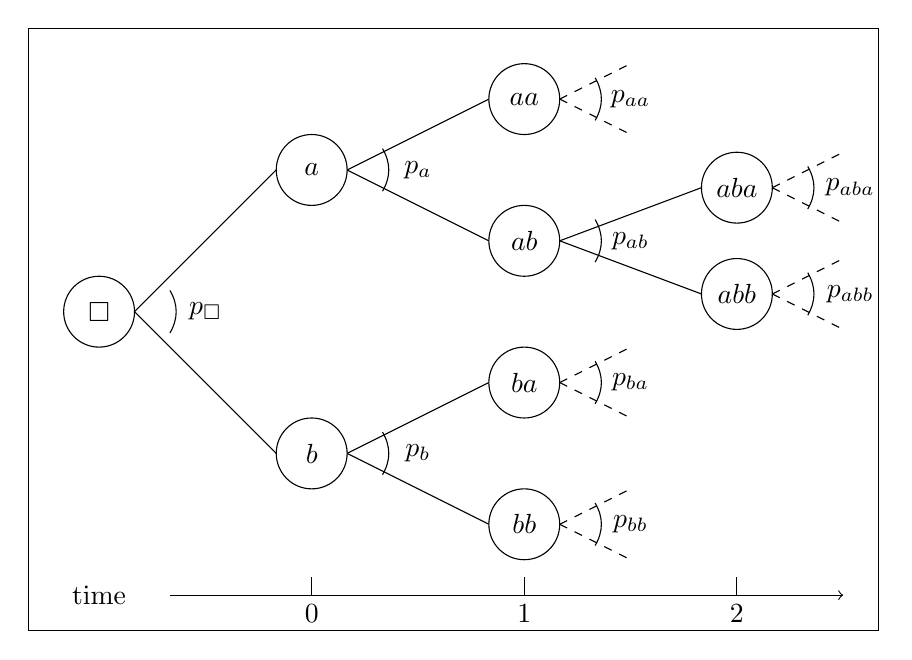
\begin{tikzpicture}[xscale=0.9,yscale=0.9]
%\draw[help lines] (-1,-0.5) grid (11,7.5);
\draw (-1,-1) rectangle (11,7.5);
\draw (0,3.5) circle(0.5) node[align=center] {$\Box$};
\draw (3,5.5) circle(0.5) node[align=center] {$a$};
\draw (3,1.5) circle(0.5) node[align=center] {$b$};
\draw (6,6.5) circle(0.5) node[align=center] {$aa$};
\draw (6,4.5) circle(0.5) node[align=center] {$ab$};
\draw (6,2.5) circle(0.5) node[align=center] {$ba$};
\draw (6,0.5) circle(0.5) node[align=center] {$bb$};
\draw (9,5.25) circle(0.5) node[align=center] {$aba$};
\draw (9,3.75) circle(0.5) node[align=center] {$abb$};
\draw (0.5,3.5) -- (2.5,5.5);
\draw (0.5,3.5) -- (2.5,1.5);
\draw (3.5,5.5) -- (5.5,6.5);
\draw (3.5,5.5) -- (5.5,4.5);
\draw (3.5,1.5) -- (5.5,2.5);
\draw (3.5,1.5) -- (5.5,0.5);
\draw (6.5,4.5) -- (8.5,5.25);
\draw (6.5,4.5) -- (8.5,3.75);
\draw [dashed] (6.5,6.5) -- (7.5,7);
\draw [dashed] (6.5,6.5) -- (7.5,6);
\draw [dashed] (6.5,2.5) -- (7.5,3);
\draw [dashed] (6.5,2.5) -- (7.5,2);
\draw [dashed] (6.5,0.5) -- (7.5,1);
\draw [dashed] (6.5,0.5) -- (7.5,0);
\draw [dashed] (9.5,5.25) -- (10.5,5.75);
\draw [dashed] (9.5,5.25) -- (10.5,4.75);
\draw [dashed] (9.5,3.75) -- (10.5,4.25);
\draw [dashed] (9.5,3.75) -- (10.5,3.25);
\draw (1.5,3.5) node[align=right] {$p_{\Box}$};
%\draw (1,3.8) .. controls (1.25,3.5) .. (1,3.2);
\draw (1,3.8) to[bend left] (1,3.2);
\draw (4.5,5.5) node[align=right] {$p_{a}$};
\draw (4,5.8) to[bend left] (4,5.2);
\draw (4.5,1.5) node[align=right] {$p_{b}$};
\draw (4,1.8) to[bend left] (4,1.2);
\draw (7.5,6.5) node[align=right] {$p_{aa}$};
\draw (7,6.8) to[bend left] (7,6.2);
\draw (7.5,4.5) node[align=right] {$p_{ab}$};
\draw (7,4.8) to[bend left] (7,4.2);
\draw (7.5,2.5) node[align=right] {$p_{ba}$};
\draw (7,2.8) to[bend left] (7,2.2);
\draw (7.5,0.5) node[align=right] {$p_{bb}$};
\draw (7,0.8) to[bend left] (7,0.2);
\draw (10.6,5.25) node[align=right] {$p_{aba}$};
\draw (10,5.55) to[bend left] (10,4.95);
\draw (10.6,3.75) node[align=right] {$p_{abb}$};
\draw (10,4.05) to[bend left] (10,3.45);
\draw (0,-0.5) node[align=center] {time};
\draw [->] (1,-0.5) -- (10.5,-0.5);
\draw (3,-0.5) -- (3,-0.25);
\draw (3, -0.5) node[align=center,below] {0};
\draw (6,-0.5) -- (6,-0.25);
\draw (6, -0.5) node[align=center,below] {1};
\draw (9,-0.5) -- (9,-0.25);
\draw (9, -0.5) node[align=center,below] {2};
\end{tikzpicture}
\caption{A (partial) event tree for a binary state-space $\states=\{a,b\}$. The vertices are situations, i.e. elements of $\states^*_\Box$, and edges are induced by the prefix order $\prec$. Dashed lines represent branches that are not shown in the figure. The tree has been augmented to a probability tree, by assigning to each $w\in\states^*$ a local model $p_w$. A time axis represents at which point in time the situations can occur.}
\label{fig:example_event_tree}
\end{figure}

Such an event tree can be turned into an intuitive representation of a stochastic process by augmenting it into a \emph{probability tree}. This is done by assigning to each situation $w\in\states^*_\Box$ in the tree a \emph{local model} $p_{w}$, which is a probability mass function on $\states$; that is, it is a map $p_w:\states\to\realsnonneg$ such that $\sum_{x\in\states}p_w(x)=1$. An example of this is again illustrated in Figure~\ref{fig:example_event_tree}.
\begin{definition}[Probability Tree]\label{def:prob_tree}
A probability tree is a tuple $(\states^*_\Box,\prec,p_{(\cdot)})$, where $\states^*_\Box$ is the set of all situations, $\prec$ is the prefix order on $\states^*_\Box$, and $p_{(\cdot)}:\states^*_\Box\times\states\to\realsnonneg$ represents all local models, so that $\sum_{x\in\states}p_w(x)=1$ for all $w\in\states^*_\Box$.
\end{definition}

The mechanism by which a stochastic process obtains a certain realisation $\omega\in\Omega$ can now be interpreted as performing a weighted, random walk along this probability tree, starting from $\Box$. Following the tree in Figure~\ref{fig:example_event_tree}, this is done as follows: from $\Box$, we transition either to $a$, with probability $p_\Box(a)$, or to $b$, with probability $p_\Box(b)$. Suppose we transition to $a$. From this new situation, the next step will take us either to $aa$, with probability $p_a(a)$, or to $ab$, with probability $p_a(b)$. Proceeding in this fashion, an infinite random walk along this tree generates a full path $\omega:\natswith\to\states$, where, for all $t\in\natswith$, the state $\omega(t)$ represents the (randomly chosen) branch that we took along the tree at the $(t+1)$-th step.

This ``path construction'' view allows us also to connect back to the measure-theoretic definition that we encountered earlier. To obtain this correspondence in one direction, fix a probability tree $(\states^*_\Box,\prec, p_{(\cdot)})$ and let $(\Omega,\mathcal{F})$ be an appropriate measurable space of discrete-time sample paths, on which we will aim to construct the measure $P$ quantifying in the measure-theoretic sense the uncertainty of the corresponding stochastic process $\{X_t\}_{t\in\natswith}$ on the resulting probability space.

We now reason intuitively by using the ``random walk'' along the probability tree. Starting from $\Box$, we transition to a first situation $x\in\states$ with probability $p_\Box(x)$. From there, we could then perform the entire infinite random walk to generate the remainder of the path. So, a different way of saying this is that, of all the random paths $\omega\in\Omega$ that could be generated, a fraction of $p_\Box(x)$ of them will start with $\omega(0)=x$. Using also the interpretation given by Corollary~\ref{cor:process_prob_is_measure}, it therefore makes sense to define the \emph{first-step marginal measure} $P^*(X_0=x) \coloneqq p_\Box(x)$ for all $x\in\states$.

Let us now consider the next step, and assume the first step down the tree resulted in a situation $x\in\states$. Then, with probability $p_x(y)$, $y\in\states$, the next situation will be $xy$. In terms of paths that could be generated, a fraction of $p_x(y)$ of the paths that satisfy $\omega(0)=x$, will furthermore satisfy $\omega(1)=y$. Therefore, we define for the \emph{second}-step marginal measure $P^*(X_0=x,X_1=y)\coloneqq p_\Box(x)p_x(y)$.

Proceeding in this manner, for every situation $w\in\states^*$ with length $n+1$, $n\in\natswith$, we can compute the $(n+1)$-th step marginal measure as
\begin{equation*}
P^*\bigl(X_{0:n}=w\bigr) \coloneqq p_\Box\bigl(w_0\bigr)\prod_{i=1}^{n} p_{w_0\cdots w_{i-1}}\bigl(w_i\bigr)\,,
\end{equation*}
or in words, by multiplying all probabilities given by the local models of the situations encountered on the path from the root of the tree, down to the situation $w$.

A fundamental result in the measure-theoretic treatment of stochastic processes (known as the \emph{Kolmogorov extension theorem}) states that the collection of all these $n$-th step marginal measures $P^*$ induces (``coherently'') a probability measure $P$ on $(\Omega,\mathcal{F})$. Specifically, the finite $n$-th step marginals of $P$ will correspond exactly to these $n$-th step marginal measures that we constructed from the probability tree. This establishes the connection between probability trees and discrete-time measure-theoretic stochastic processes, in that the latter can be constructed from the former.

For the other direction, so, to construct a probability tree from a given probability space $(\Omega,\mathcal{F},P)$, we start with an event tree $(\states^*_\Box,\prec)$ and aim to construct the local models $p_{(\cdot)}$. Using the intuitive interpretation offered by Corollary~\ref{cor:process_prob_is_measure}, we start by setting $p_\Box(x)=P(X_0=x)$ for all $x\in\states$. For all other situations $w\in\states^*$ with length $n+1$, $n\in\natswith$, the local model $p_w$ is defined as the conditional measure constructed from Bayes' rule, i.e., for all $x\in\states$,
\begin{align*}
p_w(x) &= P\bigl( X_{n+1}=x\,\big\vert\, X_{0:n}=w \bigr) = \frac{P\bigl(X_{0:n}=w, X_{n+1}=x\bigr)}{P\bigl( X_{0:n}=w \bigr)}\,.
\end{align*}
This also establishes the connection in the other direction. It can be verified that, by now constructing from this probability tree a measure $P^*$, say, in the manner described above, we obtain again $P^*=P$; so, we conclude that this yields a one-to-one correspondence between probability trees and measure-theoretic stochastic processes.

It should be noted that the second direction in the preceding discussion has one (rather large) caveat: it does not work when there are partial paths that have zero probability to occur. This is because then Bayes' rule cannot define the conditional measure required to construct the local model for the situation corresponding to that partial path, since it would result in a division by zero.

To summarise, we can conclude that there is indeed a correspondence between the two representations that we have seen so far (up to some technical difficulties surrounding probabilities that are zero). We have seen that the graphical tree structure allows us to reason intuitively about how a stochastic process generates a sample path, by ``walking'' from the root of the tree down its branches. As we will discuss next, we can also use this structure to ``reason backwards'': from vertices deep down in the tree back to the root. We will see that this allows one to intuitively derive \emph{computational methods} for working with stochastic processes. 

So, fix $n\in\natswith$ and let $f\in\gambles(\states^{n+1})$ be a real-valued function of which we aim to compute the expected value with respect to the random variables $X_{0:n}$ at the time points $0,\ldots,n\in\natswith$. Note that it suffices to consider this case, in the sense that any function defined on a subset of the variables $X_{0:n}$, can always be trivially extended to a function on all of them. Now first notice the following. For any situation $w\in\states^*$ with length $\lvert w\rvert = n+1$, the value of $f$ in $w$ is easy to compute; it is simply $f(w)$. Hence in particular, the \emph{expected value} of $f$, in $w$, is simply
\begin{equation*}
\mathbb{E}\bigl[f(X_{0:n})\,\big\vert\,X_{0:n}=w\bigr] = f(w)\,.
\end{equation*}
Recall that the situation $w$ represents a node in the event tree. We will now ``pull back'' the above expected value, to the time-point $n$. Consider therefore the parent situation of $w$ in the probability tree; we will compute the expected value of $f$ in this parent situation.

This parent is a situation $v$ of length $\lvert v\lvert=\lvert w\lvert-1=n$, which entirely coincides with $w$: $v_i=w_i$ for all $i=0,\ldots,n-1$. Associated to $v$ is the local probability model $p_v$ which, as we have discussed above, represents the probability with which a random walk along the tree travels through the various children of $v$. In particular, such a random walk goes through the situation $w$, with probability $p_v(w_\top)$. Therefore, the contribution of the expected value in $w$, to the expected value in $v$, is the expected value in $w$ weighted by $p_v(w_\top)$. Since this holds for all children of $v$, we can write
\begin{align*}
&\mathbb{E}\bigl[f(X_{0:n}) \,\big\vert\, X_{0:(n-1)}=v \bigr] = \sum_{x\in\states} p_v(x)\mathbb{E}\bigl[f(X_{0:n})\,\big\vert\,X_{0:(n-1)}=v,X_n=x\bigr]\,.
\end{align*}
This ``pullback'' operation is graphically illustrated in Figure~\ref{fig:pullback_loie}.

\begin{figure}
\centering
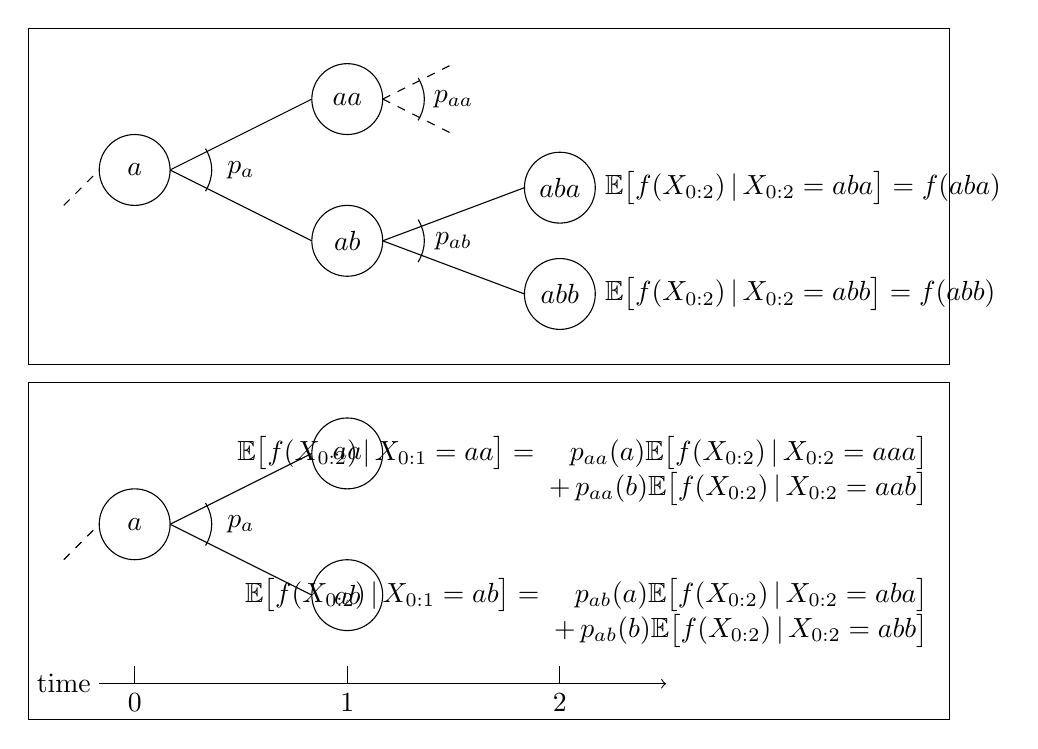
\begin{tikzpicture}[xscale=0.9,yscale=0.9]
%\draw[help lines] (-1,-0.5) grid (11,7.5);
\draw (-0.5,2.75) rectangle (12.5,7.5);
\draw (1,5.5) circle(0.5) node[align=center] {$a$};
\draw (4,6.5) circle(0.5) node[align=center] {$aa$};
\draw (4,4.5) circle(0.5) node[align=center] {$ab$};
\draw (7,5.25) circle(0.5) node[align=center] {$aba$};
\draw (7,3.75) circle(0.5) node[align=center] {$abb$};
\draw [dashed] (0,5) -- (0.5,5.5);
\draw (1.5,5.5) -- (3.5,6.5);
\draw (1.5,5.5) -- (3.5,4.5);
\draw (4.5,4.5) -- (6.5,5.25);
\draw (4.5,4.5) -- (6.5,3.75);
\draw [dashed] (4.5,6.5) -- (5.5,7);
\draw [dashed] (4.5,6.5) -- (5.5,6);
\draw (2.5,5.5) node[align=right] {$p_{a}$};
\draw (2,5.8) to[bend left] (2,5.2);
\draw (5.5,6.5) node[align=right] {$p_{aa}$};
\draw (5,6.8) to[bend left] (5,6.2);
\draw (5.5,4.5) node[align=right] {$p_{ab}$};
\draw (5,4.8) to[bend left] (5,4.2);
\draw (7.5,5.25) node[anchor=west] {$\mathbb{E}\bigl[f(X_{0:2})\,\vert\,X_{0:2}=aba\bigr]=f(aba)$};
\draw (7.5,3.75) node[anchor=west] {$\mathbb{E}\bigl[f(X_{0:2})\,\vert\,X_{0:2}=abb\bigr]=f(abb)$};
%
%
\draw (-0.5,-2.25) rectangle (12.5,2.5);
\draw (1,0.5) circle(0.5) node[align=center] {$a$};
\draw (4,1.5) circle(0.5) node[align=center] {$aa$};
\draw (4,-0.5) circle(0.5) node[align=center] {$ab$};
\draw [dashed] (0,0) -- (0.5,0.5);
\draw (1.5,0.5) -- (3.5,1.5);
\draw (1.5,0.5) -- (3.5,-0.5);
\draw (2.5,0.5) node[align=right] {$p_{a}$};
\draw (2,0.8) to[bend left] (2,0.2);
%\draw (4.5,1.5) node[anchor=west] {$\mathbb{E}\bigl[f(X_{0:2})\,\vert\,X_{0:1}=aa\bigr]$};
\draw (12.33,1.5) node[anchor=east] {$\mathbb{E}\bigl[f(X_{0:2})\,\vert\,X_{0:1}=aa\bigr]= \quad p_{aa}(a)\mathbb{E}\bigl[f(X_{0:2})\,\vert\,X_{0:2}=aaa\bigr]$};
\draw (12.33,1) node[anchor=east] {$+\,  p_{aa}(b)\mathbb{E}\bigl[f(X_{0:2})\,\vert\,X_{0:2}=aab\bigr]$};
\draw (12.33,-0.5) node[anchor=east] {$\mathbb{E}\bigl[f(X_{0:2})\,\vert\,X_{0:1}=ab\bigr]= \quad p_{ab}(a)\mathbb{E}\bigl[f(X_{0:2})\,\vert\,X_{0:2}=aba\bigr]$};
\draw (12.33,-1) node[anchor=east] {$+\,  p_{ab}(b)\mathbb{E}\bigl[f(X_{0:2})\,\vert\,X_{0:2}=abb\bigr]$};
%\draw (4.62,2.5) -- (4.62,-1.5);
\draw (0,-1.75) node[align=center] {time};
\draw [->] (0.5,-1.75) -- (8.5,-1.75);
\draw (1,-1.75) -- (1,-1.5);
\draw (1, -1.75) node[align=center,below] {0};
\draw (4,-1.75) -- (4,-1.5);
\draw (4, -1.75) node[align=center,below] {1};
\draw (7,-1.75) -- (7,-1.5);
\draw (7, -1.75) node[align=center,below] {2};
\end{tikzpicture}
\caption{Graphical illustration of ``pulling back'' the expected value of a function $f$ on $X_{0:2}$, in a probability tree on a binary state-space $\states=\{a,b\}$. Top: the function $f$ is entirely determined by the situations of length 3, i.e. the expected value of the function in those situations, is simply the value of the function evaluated in that situation. Bottom: result after ``pulling back'' the expectations by one step. The resulting conditional expectation is a function whose value is entirely determined by the situations of length 2. The values are the weighted average of the expectations in the child nodes, weighted by the local models $p_{(\cdot)}$.}
\label{fig:pullback_loie}
\end{figure}

Now, observe that the above conditional expectation of $f$ in $v$, is itself a real-valued function in $\gambles(\states^n)$. Its value is determined by the states at times $0,\ldots,n-1$. We can therefore repeat the above argument; we pull back to the parent of $v$, then to the parent of \emph{that} situation, and so on. Eventually, the parent that we are considering is the empty situation $\Box$; we then finish by computing
\begin{equation*}
\mathbb{E}\bigl[f(X_{0:n})\bigr] = \sum_{x\in\states} p_\Box(x) \mathbb{E}\bigl[f(X_{0:n})\,\big\vert\,X_0=x\bigr]\,,
\end{equation*}
which is exactly the expected value of $f$ that we started out wanting to compute.

This method to compute the expected value of a function by ``pulling back'' the ``local'', or conditional, expected values, uses the interpretation of a stochastic process as a probability tree. The method relies on a property that is called the \emph{law of iterated expectation}, or alternatively the \emph{law of total probability}. It can be stated formally in the measure-theoretic context, where it is also easily stated for \emph{continuous}-time stochastic processes.
\begin{theorem}\label{thm:loie}
Fix a time-dimension $\timedim\in\{\natswith,\realsnonneg\}$, and let $\{X_t\}_{t\in\timedim}$ be a stochastic process on $(\Omega,\mathcal{F},P)$. Choose any three ordered sequences $\mathbf{s}=s_1,\ldots,s_n$, $\mathbf{t}=t_1,\ldots,t_m$, and $\mathbf{u}=u_1,\ldots,u_\ell$ in $\timedim$, with $n,m,\ell\in\nats$ such that $s_n<t_1$ and $t_m<u_1$. Then for any real-valued function $f\in\gambles(\states^{n+m+\ell})$ on $X_\mathbf{s},X_\mathbf{t},X_\mathbf{u}$, it holds that
\begin{equation*}
\mathbb{E}\bigl[f(X_\mathbf{s},X_\mathbf{t},X_\mathbf{u})\,\big\vert\,X_\mathbf{s}\bigr] = \mathbb{E}\Bigl[\mathbb{E}\bigl[f(X_\mathbf{s},X_\mathbf{t},X_\mathbf{u})\,\big\vert\,X_\mathbf{s},X_\mathbf{t}\bigr]\,\Big\vert\,X_\mathbf{s}\Bigr]\,,
\end{equation*} 
whenever $P(X_\mathbf{s})$ and $P(X_\mathbf{s},X_\mathbf{t})$ are everywhere strictly positive.
\end{theorem}

Having discussed how to interpret probability trees, and how to use them to reason about the computation of expected values, we now move on to a discussion of their structural properties. Note that the specification of a probability tree is still relatively complicated. This is not really due to the structure of the tree; the situations $\states^*_\Box$ and prefix order $\prec$ carry enough information to construct the tree up to any desired level, and their mathematical specification is straightforward. However, in order to specify all the local models $p_{(\cdot)}$, we need to provide an infinite number of probability mass functions on $\states$; one for each situation $w\in\states^*_\Box$. This is why one often restricts attention to simpler models, where one needs less, and often only finitely many, local models.

These simplifications can be seen as a matter of degree. At the one extreme, we have the general definition that we used above, where each situation $w\in\states^*_\Box$ has a local model $p_w$. This leads to a lot of possible structure, but is hard to specify. At the other extreme is the \emph{independent and identically distributed} (i.i.d.) process; this is when we only have a single probability mass function $p$, and we set $p_w\coloneqq p$ for all $w\in\states^*_\Box$. For such a process, no matter what situation we are in, the next branch will always be chosen according to $p$. This process is easy to specify, but it does not yield a lot of structure that can capture the dynamics of the underlying system that we are trying to model.

A useful step up from the i.i.d. process is reached by the popular class of models known as \emph{homogeneous Markov chains}. For a homogeneous Markov chain, the local model \emph{only} depends on the last step of the corresponding situation, and not on what happened before that:
\begin{definition}[Homogeneous Markov Chain as Probability Tree]\label{def:prob_tree_homogen_markov}
A probability tree $(\states^*_\Box,\prec,p_{(\cdot)})$ is called a homogeneous Markov chain if, for all situations $v,w\in\states^*$ such that $v_\top=w_\top$, it holds that $p_v=p_w$.
\end{definition} 
\begin{corollary}
Let $(\states^*_\Box,\prec,p_{(\cdot)})$ be a homogeneous Markov chain. Then for all $x\in\states$ and all $w\in\states^*$ such that $w_\top=x$, it holds that $p_w=p_x$.
\end{corollary}
\begin{proof}
Trivial from Definition~\ref{def:prob_tree_homogen_markov} and the fact that all $x\in\states$ are also situations. 
\end{proof}
\begin{figure}
\centering
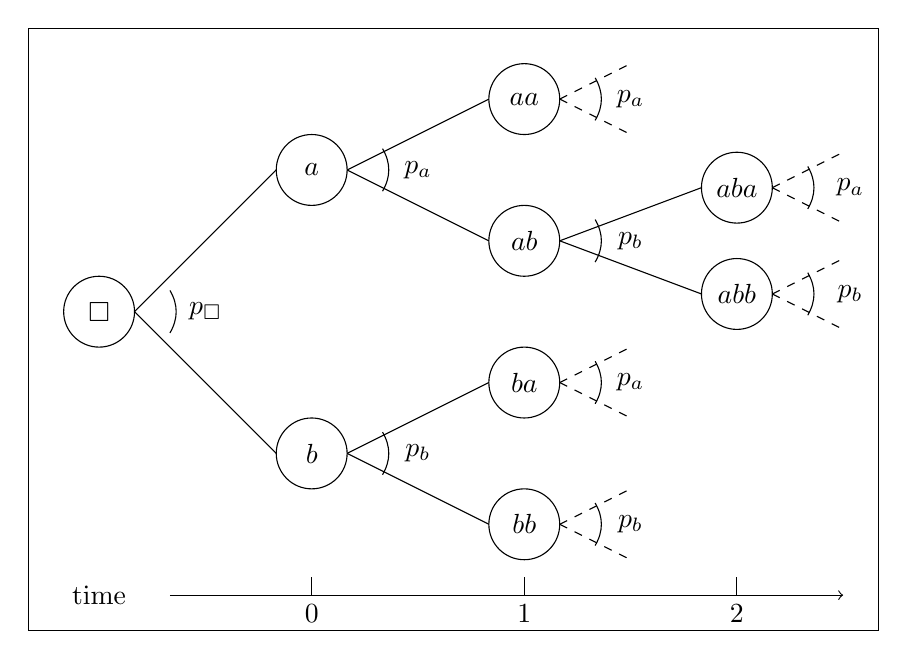
\begin{tikzpicture}[xscale=0.9,yscale=0.9]
%\draw[help lines] (-1,-0.5) grid (11,7.5);
\draw (-1,-1) rectangle (11,7.5);
\draw (0,3.5) circle(0.5) node[align=center] {$\Box$};
\draw (3,5.5) circle(0.5) node[align=center] {$a$};
\draw (3,1.5) circle(0.5) node[align=center] {$b$};
\draw (6,6.5) circle(0.5) node[align=center] {$aa$};
\draw (6,4.5) circle(0.5) node[align=center] {$ab$};
\draw (6,2.5) circle(0.5) node[align=center] {$ba$};
\draw (6,0.5) circle(0.5) node[align=center] {$bb$};
\draw (9,5.25) circle(0.5) node[align=center] {$aba$};
\draw (9,3.75) circle(0.5) node[align=center] {$abb$};
\draw (0.5,3.5) -- (2.5,5.5);
\draw (0.5,3.5) -- (2.5,1.5);
\draw (3.5,5.5) -- (5.5,6.5);
\draw (3.5,5.5) -- (5.5,4.5);
\draw (3.5,1.5) -- (5.5,2.5);
\draw (3.5,1.5) -- (5.5,0.5);
\draw (6.5,4.5) -- (8.5,5.25);
\draw (6.5,4.5) -- (8.5,3.75);
\draw [dashed] (6.5,6.5) -- (7.5,7);
\draw [dashed] (6.5,6.5) -- (7.5,6);
\draw [dashed] (6.5,2.5) -- (7.5,3);
\draw [dashed] (6.5,2.5) -- (7.5,2);
\draw [dashed] (6.5,0.5) -- (7.5,1);
\draw [dashed] (6.5,0.5) -- (7.5,0);
\draw [dashed] (9.5,5.25) -- (10.5,5.75);
\draw [dashed] (9.5,5.25) -- (10.5,4.75);
\draw [dashed] (9.5,3.75) -- (10.5,4.25);
\draw [dashed] (9.5,3.75) -- (10.5,3.25);
\draw (1.5,3.5) node[align=right] {$p_{\Box}$};
%\draw (1,3.8) .. controls (1.25,3.5) .. (1,3.2);
\draw (1,3.8) to[bend left] (1,3.2);
\draw (4.5,5.5) node[align=right] {$p_{a}$};
\draw (4,5.8) to[bend left] (4,5.2);
\draw (4.5,1.5) node[align=right] {$p_{b}$};
\draw (4,1.8) to[bend left] (4,1.2);
\draw (7.5,6.5) node[align=right] {$p_{a}$};
\draw (7,6.8) to[bend left] (7,6.2);
\draw (7.5,4.5) node[align=right] {$p_{b}$};
\draw (7,4.8) to[bend left] (7,4.2);
\draw (7.5,2.5) node[align=right] {$p_{a}$};
\draw (7,2.8) to[bend left] (7,2.2);
\draw (7.5,0.5) node[align=right] {$p_{b}$};
\draw (7,0.8) to[bend left] (7,0.2);
\draw (10.6,5.25) node[align=right] {$p_{a}$};
\draw (10,5.55) to[bend left] (10,4.95);
\draw (10.6,3.75) node[align=right] {$p_{b}$};
\draw (10,4.05) to[bend left] (10,3.45);
\draw (0,-0.5) node[align=center] {time};
\draw [->] (1,-0.5) -- (10.5,-0.5);
\draw (3,-0.5) -- (3,-0.25);
\draw (3, -0.5) node[align=center,below] {0};
\draw (6,-0.5) -- (6,-0.25);
\draw (6, -0.5) node[align=center,below] {1};
\draw (9,-0.5) -- (9,-0.25);
\draw (9, -0.5) node[align=center,below] {2};
\end{tikzpicture}
\caption{A homogeneous Markov chain, represented as a probability tree.}
\label{fig:example_homogen_markov_tree}
\end{figure}
An example for the binary state space $\states=\{a,b\}$ is shown in Figure~\ref{fig:example_homogen_markov_tree}. Additional degrees of freedom can be introduced back into this model by also letting the local models depend on the corresponding depth of the tree. The dynamics can then depend on the point in time, but not on the \emph{specific} history up to that time. This yields the more general definition of a (non-homogeneous) \emph{Markov chain}:
\begin{definition}[Markov Chain as Probability Tree]\label{def:prob_tree_markov}
A probability tree $(\states^*_\Box,\prec,p_{(\cdot)})$ is called a Markov chain if, for all situations $v,w\in\states^*$ for which $\lvert v\rvert=\lvert w\rvert$ and $v_\top=w_\top$, it holds that $p_v=p_w$.
\end{definition}
\begin{figure}
\centering
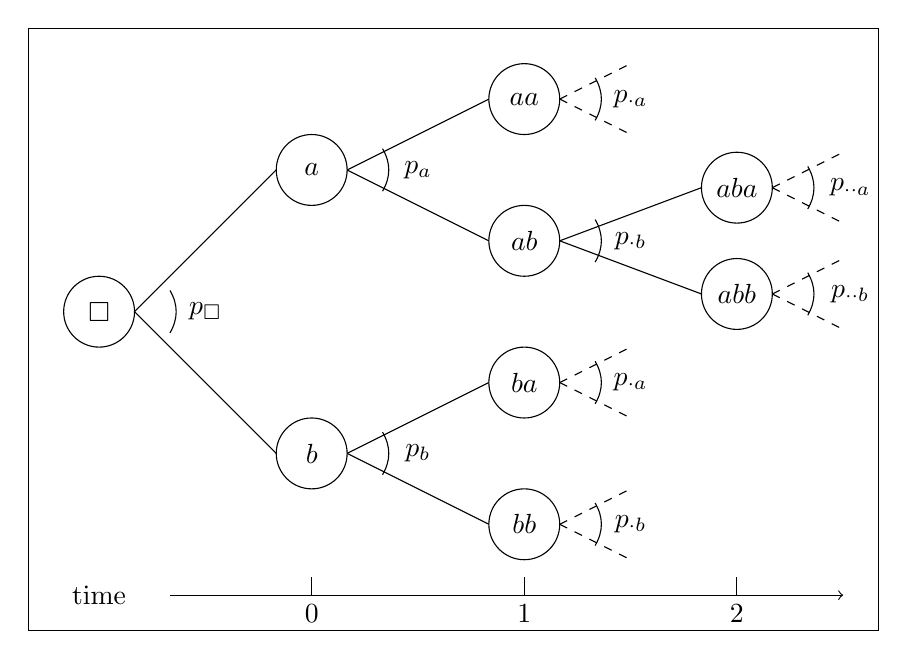
\begin{tikzpicture}[xscale=0.9,yscale=0.9]
%\draw[help lines] (-1,-0.5) grid (11,7.5);
\draw (-1,-1) rectangle (11,7.5);
\draw (0,3.5) circle(0.5) node[align=center] {$\Box$};
\draw (3,5.5) circle(0.5) node[align=center] {$a$};
\draw (3,1.5) circle(0.5) node[align=center] {$b$};
\draw (6,6.5) circle(0.5) node[align=center] {$aa$};
\draw (6,4.5) circle(0.5) node[align=center] {$ab$};
\draw (6,2.5) circle(0.5) node[align=center] {$ba$};
\draw (6,0.5) circle(0.5) node[align=center] {$bb$};
\draw (9,5.25) circle(0.5) node[align=center] {$aba$};
\draw (9,3.75) circle(0.5) node[align=center] {$abb$};
\draw (0.5,3.5) -- (2.5,5.5);
\draw (0.5,3.5) -- (2.5,1.5);
\draw (3.5,5.5) -- (5.5,6.5);
\draw (3.5,5.5) -- (5.5,4.5);
\draw (3.5,1.5) -- (5.5,2.5);
\draw (3.5,1.5) -- (5.5,0.5);
\draw (6.5,4.5) -- (8.5,5.25);
\draw (6.5,4.5) -- (8.5,3.75);
\draw [dashed] (6.5,6.5) -- (7.5,7);
\draw [dashed] (6.5,6.5) -- (7.5,6);
\draw [dashed] (6.5,2.5) -- (7.5,3);
\draw [dashed] (6.5,2.5) -- (7.5,2);
\draw [dashed] (6.5,0.5) -- (7.5,1);
\draw [dashed] (6.5,0.5) -- (7.5,0);
\draw [dashed] (9.5,5.25) -- (10.5,5.75);
\draw [dashed] (9.5,5.25) -- (10.5,4.75);
\draw [dashed] (9.5,3.75) -- (10.5,4.25);
\draw [dashed] (9.5,3.75) -- (10.5,3.25);
\draw (1.5,3.5) node[align=right] {$p_{\Box}$};
%\draw (1,3.8) .. controls (1.25,3.5) .. (1,3.2);
\draw (1,3.8) to[bend left] (1,3.2);
\draw (4.5,5.5) node[align=right] {$p_{a}$};
\draw (4,5.8) to[bend left] (4,5.2);
\draw (4.5,1.5) node[align=right] {$p_{b}$};
\draw (4,1.8) to[bend left] (4,1.2);
\draw (7.5,6.5) node[align=right] {$p_{\cdot a}$};
\draw (7,6.8) to[bend left] (7,6.2);
\draw (7.5,4.5) node[align=right] {$p_{\cdot b}$};
\draw (7,4.8) to[bend left] (7,4.2);
\draw (7.5,2.5) node[align=right] {$p_{\cdot a}$};
\draw (7,2.8) to[bend left] (7,2.2);
\draw (7.5,0.5) node[align=right] {$p_{\cdot b}$};
\draw (7,0.8) to[bend left] (7,0.2);
\draw (10.6,5.25) node[align=right] {$p_{\cdot\cdot a}$};
\draw (10,5.55) to[bend left] (10,4.95);
\draw (10.6,3.75) node[align=right] {$p_{\cdot\cdot b}$};
\draw (10,4.05) to[bend left] (10,3.45);
\draw (0,-0.5) node[align=center] {time};
\draw [->] (1,-0.5) -- (10.5,-0.5);
\draw (3,-0.5) -- (3,-0.25);
\draw (3, -0.5) node[align=center,below] {0};
\draw (6,-0.5) -- (6,-0.25);
\draw (6, -0.5) node[align=center,below] {1};
\draw (9,-0.5) -- (9,-0.25);
\draw (9, -0.5) node[align=center,below] {2};
\end{tikzpicture}
\caption{A (non-homogeneous) Markov chain, represented as a probability tree.}
\label{fig:example_markov_tree}
\end{figure}
An example for the binary state space $\states=\{a,b\}$ is shown in Figure~\ref{fig:example_markov_tree}. It can be verified that a homogeneous Markov chain is a Markov chain, but not---in general---the other way around. 
Note that, in contrast to homogeneous Markov chains where we only needed to specify local models $p_x$ for all $x\in\states$, we now need different local models for each level of the tree. So, we are now back to needing an infinite number of local models in order to fully describe such a model.

These definitions of (homogeneous) Markov chains can also be conveniently translated back to the measure-theoretic context. We here give the general definition, for an arbitrary time-dimension (so, either $\timedim=\natswith$ or $\timedim=\realsnonneg$) and multiple steps into the future:
\begin{definition}[Markov Chain as Probability Measure]\label{def:measure_markov}
A stochastic process $\{X_t\}_{t\in\timedim}$ on $(\Omega,\mathcal{F},P)$ is called a Markov chain if for all $s_1,\ldots,s_n,t\in\timedim$, $n\in\nats$, such that $s_1<\cdots<s_n<t$, it holds that $P(X_t\,\vert\,X_{s_1},\ldots,X_{s_n}) = P(X_t\,\vert\,X_{s_n})$. A stochastic process that is a Markov chain, is said to have the Markov property.
\end{definition}
Similarly, the notion of homogeneity can be defined measure-theoretically and for an arbitrary time-dimension:  
\begin{definition}[Homogeneous Markov Chain as Probability Measure]\label{def:measure_homogen_markov}
A stochastic process $\{X_t\}_{t\in\timedim}$ on $(\Omega,\mathcal{F},P)$ is called a homogeneous Markov chain if it is a Markov chain, and if additionally, for all $s,t\in\timedim$ such that $s<t$, it holds that $P(X_t\,\vert\,X_s)=P(X_{t-s}\,\vert\,X_0)$.
\end{definition}
We leave it as an exercise to verify that, when $\timedim=\natswith$, Definitions~\ref{def:measure_markov} and~\ref{def:measure_homogen_markov} correspond to what we would expect from Definitions~\ref{def:prob_tree_markov} and~\ref{def:prob_tree_homogen_markov}, respectively.

\subsection{Probabilistic Graphical Models}

We now move on to a different graphical representation of stochastic processes, that is useful for discrete-time Markov chains in particular: \emph{probabilistic graphical models} (PGMs), which are also known as \emph{Bayesian networks}. While the graphical structure of probability trees in Section~\ref{sec:prob_trees} emphasised the partial paths in the realisation of a stochastic process, the PGM representation emphasises the individual random variables $X_t$. 

The PGM representation of a discrete-time Markov chain $\{X_t\}_{t\in\natswith}$ is given in Figure~\ref{fig:example_markov_pgm}. The structure is a directed acyclic graph, with one node associated to each random variable $X_t$, and arcs representing the dependence of the receiving node's random variable's distribution, on the originating node's random variable's value. Due to the Markov property (c.f. Definition~\ref{def:measure_markov}), each random variable $X_n$, $n\in\nats$, is only influenced by $X_{n-1}$, the value of the random variable immediately before it. The initial variable $X_0$ is somewhat of a special case, since it does not depend on any other variables; there are no time-points preceding it. Due to these properties, the graphical structure is that of a chain; this may go some way in explaining the name ``Markov chain''. In the remainder of this section, we will refer to both a node in the PGM and to its random variable, using the same notation $X_t$.
\begin{figure}
\centering
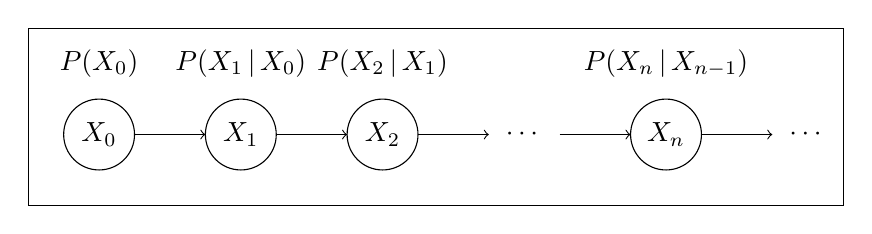
\begin{tikzpicture}[xscale=0.9,yscale=0.9]
%\draw[help lines] (-1,-0.5) grid (11,7.5);
\draw (-1,-1) rectangle (10.5,1.5);
\draw (0,0) circle(0.5) node[align=center] {$X_0$};
\draw (0,1) node[align=right] {$P(X_0)$};
\draw [->] (0.5,0) -- (1.5,0);
\draw (2,0) circle(0.5) node[align=center] {$X_1$};
\draw (2,1) node[align=right] {$P(X_1\,\vert\,X_0)$};
\draw [->] (2.5,0) -- (3.5,0);
\draw (4,0) circle(0.5) node[align=center] {$X_2$};
\draw (4,1) node[align=right] {$P(X_2\,\vert\,X_1)$};
\draw [->] (4.5,0) -- (5.5,0);
\draw (6,0) node[align=right] {$\cdots$};
\draw [->] (6.5,0) -- (7.5,0);
\draw (8,0) circle(0.5) node[align=center] {$X_n$};
\draw (8,1) node[align=right] {$P(X_n\,\vert\,X_{n-1})$};
\draw [->] (8.5,0) -- (9.5,0);
\draw (10,0) node[align=right] {$\cdots$};
\end{tikzpicture}
\caption{Probabilistic graphical model representation of a discrete-time Markov chain $\{X_t\}_{t\in\natswith}$. Nodes represent random variables. An incoming arc on a node represents that the distribution of the corresponding random variable is influenced by the originating node of that arc. Correspondingly, each node associates a probability distribution to its random variable, conditional on the values of the random variables of the nodes by which it is influenced.}
\label{fig:example_markov_pgm}
\end{figure}

It should be emphasised that the graphical structure is not saying that only nodes which are adjacent in the PGM can influence each other. The formal interpretation is as follows: for any node $X_n$, $n\in\nats$, \emph{conditional on the value of the parent(s) of $X_n$}, the distribution of $X_n$ is probabilistically independent of the non-parents, non-descendants of $X_n$. This is the general interpretation of the independence properties of the arcs in a PGM. In the special case of Markov chains that we are considering here, the interpretation vastly simplifies. Notably, the ``non-parents, non-descendants'' of any node $X_n$ are exactly its ``grand-parents'', ``great-grand-parents'', and so on; it is the set of nodes $\{X_{m}\,:\,m\in\natswith,\, m<n-1\}$.

Put differently, the value of $X_n$ influences the distribution of \emph{all} of its descendants (i.e. the nodes $X_m$, $m>n$), so long as we do not know the value of any of those descendants themselves. We will next consider how to can quantify this.

We start by observing that for each node $X_n$, $n\in\nats$, we have the associated conditional probability $P(X_n\,\vert\,X_{n-1})$. Since the state-space $\states$ is taken to be finite, we can conveniently represent these conditional probabilities in a $\lvert\states\rvert\times\lvert\states\rvert$ matrix. For any $t\in\natswith$, this matrix $T_t$ is defined, for all $x,y\in\states$, as
\begin{equation*}
T_t(x,y) \coloneqq P(X_{t+1}=y\,\vert\,X_t=x)\,,
\end{equation*}
where the indexing is taken to be row-first. This matrix $T_t$ is called the \emph{transition matrix} of the Markov chain at time $t$. Its elements $T_t(x,y)$ are called the \emph{transition probabilities from $x$ to $y$}, and they are the probabilities that a system that is in state $x$ at time $t$, will be in state $y$ at time $t+1$. This explains the subscript-indexing, whereby the matrix $T_t$ contains the conditional probabilities associated to node $X_{t+1}$.

The reason that we represent these probabilities using matrices is that this opens up the entire toolbox of linear algebra. We will see that this allows us to very succinctly write down certain relations and properties. For instance, we can now write the influence of a node on its descendants, using a simple matrix product:
\begin{proposition}\label{prop:markov_factor_transmat}
Let $\{X_t\}_{t\in\natswith}$ be a discrete-time Markov chain, and let $T_t$ be the associated family of transition matrices, as defined above. Then for all $s,t\in\natswith$ such that $s\leq t$, and all $x,y\in\states$, it holds that $P(X_{t+1}=y\,\vert\,X_s=x) = \left[T_s\cdots T_{t}\right](x,y)$.
\end{proposition}
\begin{proof}
We give a proof by induction. For $t=s$ the result is immediate from the definition of the transition matrix $T_s$. Now suppose the result is true for $t-1$; we show that it is also true for $t$:
\begin{align*}
P(X_{t+1}=y\,\vert\,X_s=x) &= \sum_{z\in\states} P(X_{t+1}=y,X_{t}=z\,\vert\,X_s=x) \\
 &= \sum_{z\in\states} P(X_{t}=z\,\vert\,X_s=x) P(X_{t+1}=y\,\vert\,X_{t}=z,\,X_s=x) \\
 &= \sum_{z\in\states} \left[T_s\cdots T_{t-1}\right](x,z) P(X_{t+1}=y\,\vert\,X_{t}=z) \\
 &= \sum_{z\in\states} \left[T_s\cdots T_{t-1}\right](x,z) T_{t}(z,y) = \bigl[T_s\cdots T_{t-1}T_{t}\bigr](x,y)\,,
\end{align*}
where the first and second equalities are basic properties of probabilities, the third equality is due to the induction hypothesis and the Markov property (c.f. Definition~\ref{def:measure_markov}), the fourth equality uses the definition of the transition matrix $T_{t}$, and the final equality uses the definition of a matrix product. 
\end{proof}

Another useful property of this representation, is that it allows us to write conditional expectations of functions $f\in\gamblesX$ using matrix-vector products. In particular, again because $\states$ is finite, any $f\in\gamblesX$ can be interpreted as a vector in $\reals^{\lvert\states\rvert}$; the coordinates are simply the values $f(x)$, $x\in\states$. Hence:
\begin{proposition}\label{prop:expectation_using_transmat}
Let $\{X_t\}_{t\in\natswith}$ be a discrete-time Markov chain, and let $T_t$ be the associated family of transition matrices. Then, for all $f\in\gamblesX$, all $t\in\natswith$, and all $x\in\states$, it holds that $\mathbb{E}\bigl[f(X_{t+1})\,\vert\,X_t=x\bigr] = \left[T_tf\right](x)$.
\end{proposition}
\begin{proof}
Simply use the definition of the matrix-vector product: 
\begin{equation*}
\left[T_tf\right](x)=\sum_{y\in\states}T_t(x,y)f(y)=\sum_{y\in\states}P(X_{t+1}=y\,\vert\,X_t=x)f(y) = \mathbb{E}\bigl[f(X_{t+1})\,\vert\,X_t=x\bigr].
\vspace{-16pt}
\end{equation*}
\end{proof}

The above properties can be combined to give a simplified version of the law of iterated expectation (Theorem~\ref{thm:loie}) that we encountered in Section~\ref{sec:prob_trees}:
\begin{corollary}\label{cor:trans_mat_loie}
Let $\{X_t\}_{t\in\natswith}$ be a discrete-time Markov chain, and let $T_t$ be the associated family of transition matrices. Then, for all $f\in\gamblesX$, all $s,t\in\natswith$ such that $s\leq t$, and all $x\in\states$, it holds that $\mathbb{E}\bigl[f(X_{t+1})\,\vert\,X_s=x\bigr] = \left[T_s\cdots T_tf\right](x)$.
\end{corollary}
\begin{proof}
Immediate from Propositions~\ref{prop:markov_factor_transmat} and~\ref{prop:expectation_using_transmat}.
\end{proof}
Note that, where the law of iterated expectation in Theorem~\ref{thm:loie} could be interpreted as ``pulling back'' in the associated probability tree, the above simplified version can additionally be interpreted as ``pulling back'' the conditional expectations in the associated PGM, through the product of the transition matrices. This is graphically represented in Figure~\ref{fig:example_loie_pgm}.
\begin{figure}
\centering
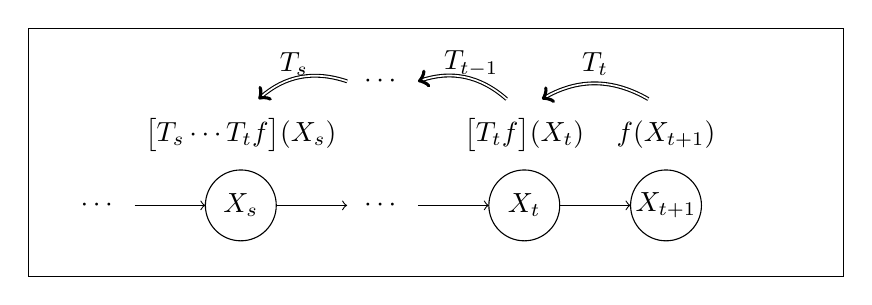
\begin{tikzpicture}[xscale=0.9,yscale=0.9]
%\draw[help lines] (-1,-0.5) grid (11,7.5);
\draw (-1,-1) rectangle (10.5,2.5);
\draw (0,0) node[align=center] {$\cdots$};
\draw [->] (0.5,0) -- (1.5,0);
\draw (2,0) circle(0.5) node[align=center] {$X_s$};
\draw (2,1) node[align=right] {$\bigl[T_s\cdots T_{t}f\bigr](X_s)$};
\draw [->] (2.5,0) -- (3.5,0);
\draw (4,0) node[align=right] {$\cdots$};
\draw [->] (4.5,0) -- (5.5,0);
\draw (6,0) circle(0.5) node[align=center] {$X_{t}$};
\draw (6,1) node[align=right] {$\bigl[T_{t}f\bigr](X_{t})$};
\draw [->] (6.5,0) -- (7.5,0);
\draw (8,0) circle(0.5) node[align=center] {$X_{t+1}$};
\draw (8,1) node[align=right] {$f(X_{t+1})$};
\draw (7,2) node[align=right] {$T_t$};
\draw (7.75,1.5) edge[->,double,bend right] (6.25,1.5);
\draw (5.25,2) node[align=right] {$T_{t-1}$};
\draw (5.75,1.5) edge[->,double,bend right] (4.5,1.75);
\draw (2.75,2) node[align=right] {$T_s$};
\draw (3.5,1.75) edge[->,double,bend right] (2.25,1.5);
\draw (4,1.75) node[align=right] {$\cdots$};
\end{tikzpicture}
\caption{Graphical representation of the ``pulling back'' interpretation of the simplified version of the law of iterated expectation in Corollary~\ref{cor:trans_mat_loie}. The function $f$, of which we want to compute the expectation on $X_{t+1}$, given $X_s$, starts at node $X_{t+1}$, where its value is trivial. The function is then ``pulled back'' to the parent $X_t$ of $X_{t+1}$, by taking the local expectation;  by left-multiplying with $T_t$. This new function $T_tf$ on $X_t$, is then ``pulled'' back by multiplying with $T_{t-1}$, and so forth. Eventually, the function $T_{s+1}\cdots T_tf$ is pulled into $X_s$, by left-multiplying with $T_s$. The resulting function on $X_s$ is the conditional expectation of interest.}
\label{fig:example_loie_pgm}
\end{figure}

\subsection{Transition Graphs}

We now move on to yet another graphical representation: the \emph{transition graph} of a homogeneous (discrete-time) Markov chain. We start by noticing the following:
\begin{proposition}
Let $\{X_t\}_{t\in\natswith}$ be a discrete-time homogeneous Markov chain, and let $T_t$ be the associated family of transition matrices. Then there is a unique matrix $T$ such that $T_t=T$ for all $t\in\natswith$. Furthermore, this matrix $T$ is row-stochastic, i.e., $T(x,y)\geq 0$ for all $x,y\in\states$, and $\sum_{y\in\states}T(x,y)=1$ for all $x\in\states$.
\end{proposition}
\begin{proof}
The matrix of interest can be identified as $T\coloneqq T_0$. Now, using the definition of a homogeneous Markov chain (Definition~\ref{def:measure_homogen_markov}) and the transition matrix $T_t$ for any $t\in\natswith$, it holds for all $x,y\in\states$ that
\begin{align*}
T(x,y) = T_0(x,y) &= P(X_1=y\,\vert\,X_0=x) \\
 &= P(X_{(t+1)-t}=y\,\vert\,X_0=x)=P(X_{t+1}=y\,\vert\,X_t=x)=T_t(x,y)\,,
\end{align*}
which concludes the proof of the first statement. The claim that $T$ is row-stochastic follows immediately from the fact that $T_0$ is.
\end{proof}

The transition graph of a discrete-time homogeneous Markov chain is a graphical representation of its associated transition matrix $T$. In this way, this representation emphasises the interactions between the \emph{states}, rather than the random variables. An example transition graph is shown in Figure~\ref{fig:example_trans_graph}. The formal definition is as follows:
\begin{definition}[Transition Graph]\label{def:trans_graph}
Let $\{X_t\}_{t\in\natswith}$ be a discrete-time homogeneous Markov chain, and let $T$ be its associated transition matrix. Then its associated \emph{transition graph} is a directed graph $(V,E)$ with one vertex for each state, $V=\states$, and, for all $x,y\in\states$, an arc $(x,y)\in E$ whenever $T(x,y)>0$.
\end{definition}
\begin{figure}
\centering
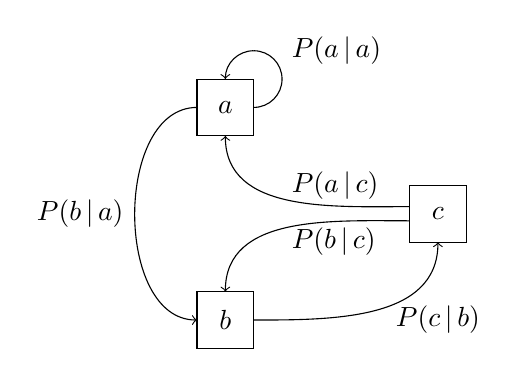
\begin{tikzpicture}[xscale=0.9,yscale=0.9]
%\draw[help lines] (-1,-0.5) grid (11,7.5);
%\draw (0,0) rectangle (10,8);
\draw (2,2) rectangle (2.8,2.8);
\draw (2.4,2.4) node[anchor=center] {$b$};
\draw (2,5) rectangle (2.8,5.8);
\draw (2.4,5.4) node[anchor=center] {$a$};
\draw (5,3.5) rectangle (5.8,4.3);
\draw (5.4,3.9) node[anchor=center] {$c$};
\draw [->] (2.8,2.4) to [out=0,in=-90] (5.4,3.5);
\draw [->] (5,3.8) to [out=180,in=90] (2.4,2.8);
\draw [->] (5,4) to [out=180,in=-90] (2.4,5);
\draw [->] (2,5.4) to [out=180,in=180] (2,2.4);
\draw (2.8,5.4) to [out=0,in=-90] (3.2,5.8);
\draw (3.2,5.8) to [out=90,in=0] (2.8,6.2);
\draw [->] (2.8,6.2) to [out=180,in=90] (2.4,5.8);
\draw (3.2,6.2) node[anchor=west] {$P(a\,\vert\,a)$};
\draw (1.1,3.9) node[anchor=east] {$P(b\,\vert\,a)$};
\draw (5.4,2.4) node {$P(c\,\vert\,b)$};
\draw (3.2,4.3) node[anchor=west] {$P(a\,\vert\,c)$};
\draw (3.2,3.5) node[anchor=west] {$P(b\,\vert\,c)$};
\end{tikzpicture}
\caption{Example transition graph for a discrete-time homogeneous Markov chain with a ternary state-space $\states=\{a,b,c\}$. The transition graph is a directed graph, with a vertex for each state, and an arc from the vertex of $x$ to that of $y$, with $x,y\in\states$, whenever $T(x,y)=P(X_1=y\,\vert\,X_0=x)>0$. The arcs are labelled with the corresponding transition probabilities. The figure uses the shorthand notation $P(y\vert x)$ for the elements $T(x,y)$ of $T$.}
\label{fig:example_trans_graph}
\end{figure}

One of the reasons transition graphs are sometimes useful, is that they allow one to study which parts of a system can be reached from other parts of the system. The simplest application is that of \emph{communicating states}:
\begin{definition}[Communicating States]\label{def:communicating_states}
Let $\{X_t\}_{t\in\natswith}$ be a discrete-time homogeneous Markov chain, and let $T$ be its associated transition matrix. For any two states $x,y\in\states$, $y$ is said to be \emph{accessible} from $x$ if there is some $n\in\nats$ such that $T^n(x,y)>0$. Furthermore, $x$ and $y$ are said to \emph{communicate} it $y$ is accessible from $x$, and $x$ is accessible from $y$. 
\end{definition}
Note that in the above, the term $T^n$ denotes the $n$-th matrix power of $T$ (c.f. Proposition~\ref{prop:markov_factor_transmat}). This has an intuitive graphical interpretation:
\begin{corollary}
Let $\{X_t\}_{t\in\natswith}$ be a discrete-time homogeneous Markov chain. Then for any $x,y\in\states$, $y$ is accessible from $x$ if and only if there is a path from $x$ to $y$ in the associated transition graph. Furthermore, $x$ and $y$ communicate if and only if there is a cycle in the associated transition graph that contains both $x$ and $y$.
\end{corollary}
\begin{proof}
Trivial from Definitions~\ref{def:trans_graph} and~\ref{def:communicating_states}.
\end{proof}
Inspection of the transition graph in Figure~\ref{fig:example_trans_graph} shows that, in that example, all states communicate with each other. A maximal set of states that all communicate with each other is called a \emph{communication class}. When a Markov chain has only a single communication class, this is called the \emph{top (communication) class}. When the top class contains all states, the Markov chain is said to be \emph{irreducible}.

Investigation of the communicating states in a Markov chain is often useful when one is interested in the long-term behaviour of the system. After all, while a system might begin in one state (or communication class), it need not necessarily always eventually return to that state (or communication class).

{\bf ** example and better introduction to the following}

An important concept is that of the \emph{regularity} of the communication classes of a Markov chain. A communication class is regular if there is a number $n\in\nats$ such that it is possible to go from any state in the class, to any other state in the class, in exactly $n$ steps. Of particular importance is the notion of \emph{top class regularity}:
\begin{definition}[Top Class Regularity]
Let $\{X_t\}_{t\in\natswith}$ be a discrete-time homogeneous Markov chain, and let $T$ be its associated transition matrix. Then the Markov chain is said to be \emph{top class regular} if
\begin{equation*}
\bigl\{ y\in\states\,:\,(\exists n\in\nats)(\forall x\in\states)\, T^n(x,y)>0 \bigr\} \neq \emptyset\,,
\end{equation*}
and in that case the top class $\states_\mathrm{top}$ of the Markov chain is equal to this set. When furthermore $\states_\mathrm{top}=\states$, the Markov chain itself is said to be \emph{regular}.
\end{definition}
The reason that this property is so important, is that it provides a sufficient condition for the long-term behaviour of a Markov chain to converge to a stationary distribution, regardless of the state in which it started:
\begin{theorem}
Let $\{X_t\}_{t\in\natswith}$ be a discrete-time homogeneous Markov chain, and let $T$ be its associated transition matrix. Let this Markov chain be regular. Then there exists a probability mass function $P_\infty:\states\to\realsnonneg$ such that, for all $x,y\in\states$, 
\begin{equation*}
P_\infty(y) = \lim_{n\to+\infty}T^n(x,y)\,.
\end{equation*}
\end{theorem}

\section{Imprecise Discrete-Time Markov Chains}

\emph{In this section: Parameterisation and imprecise local models. Different independence concepts. Different representations; sets of precise processes, (imprecise) event trees, imprecise graphical models. Computation using law of iterated lower expectation. Results on limit behaviour.}

{\bf TODO: transition better into this section. }

We will now move on to the discussion surrounding \emph{Imprecise (Discrete-Time) Markov Chains} (IDTMC). So, we still consider the time-dimension $\timedim=\natswith$. 

{\bf TODO: Sets of precise processes. Lower expectation definition. Imprecise Markov condition.}


Recall that for precise probability trees, we associate with each situation $w\in\states^*_\Box$ a local model $p_w$, which is a probability mass function on $\states$. In contrast, in order to define \emph{imprecise} probability trees, we will consider \emph{imprecise local models}. Such an imprecise local model $\mathcal{P}_w$ is simply a \emph{set} of probability mass functions on $\states$. This leads to the following definition:
\begin{definition}[Imprecise Probability Tree]
An imprecise probability tree is a tuple $(\states^*_\Box,\prec,\mathcal{P}_{(\cdot)})$, where $(\states^*_\Box,\prec)$ is an event tree, and $\mathcal{P}_{(\cdot)}$ is a set-valued function such that, for all $w\in\states^*_\Box$, $\mathcal{P}_w$ is a set of probability mass functions on $\states$.
\end{definition}
As before, the need to specify these (imprecise) local models $\mathcal{P}_w$ for all situations $w\in\states^*_\Box$ makes such a model difficult to work with. Attention is therefore restricted to \emph{imprecise Markov chains}; note that here and in what follows, we will assume the analogue of homogeneity to hold implicitly:
\begin{definition}[IDTMC as Imprecise Probability Tree]An imprecise probability tree $(\states^*_\Box,\prec,\mathcal{P}_w)$ is called an imprecise discrete-time Markov chain if, for all $v,w\in\states^*$ for which $v_\top=w_\top$, it holds that $\mathcal{P}_v=\mathcal{P}_w$.
\end{definition}

{\bf TODO: LoILE for imprecise prob trees}

{\bf TODO: Imprecise graphical models. Lower transition operators. LoILE in operator concatenation form. }

\section{Imprecise Continuous-Time Markov Chains}

\emph{In this section: Intuition as limit of discrete-time (imprecise) Markov chains. Paramerisation using local models and the (imprecise) matrix exponential. Recollection and translation of the different independence concepts. Different representations; sets of precise processes and imprecise graphical models. Reduction of computations to discrete-time case, and law of iterated lower expectation. Results on limit behaviour.}

\section{Further Reading}

\emph{In this section: Brief summary of main points including pointers to further reading. Also references to related work that we did not cover, e.g. the martingale-theoretic approach.}

\end{document}
